\chapter{Introduction}
\label{cp.intro}


From ancient times to the modern day, astronomy has played an important role in all cultures and eras.
Questions about the nature of the infinite cosmos and our place in it have intrigued great minds for millennia.
In researching the cosmos, astrophysicists try to comprehend the vast scale of the universe, both spatial and temporally.
Astronomers try to develop instruments that can tap into this ocean of cosmic data and make sense of the flood of information that results.
Each new drop of cosmic data obtained improves our understanding of the universe.

In this section, we briefly review the impact of data driven astronomy, from our understanding of stellar physics, to black holes and exoplanets. 
These discussions will lead us to open questions and build the motivation for the remainder of the thesis.


\section{Observational HR-Diagrams through the ages}

In 1872, astronomers began recording spectroscopic data for thousands of stars in the Henry Draper Catalogue~\citeme.
Antonia Maury, a female astronomer working in the observatory, noticed that some stars in the catalog were much brighter than other stars of the same color, and sorted those brighter stars into a different category from their less-luminous brethren.

Several years later, Einjar Hertzpsrung, working on his own star classification project in 1905, noticed the same thing she had: some stars had very similar colors but very different brightness~\citeme.
When he found that Maury had accounted for that in her catalog, he used it as a reference for his work.

With more data availible in 1913, Henry Norris Russell demonstrated the effect far more strikingly. 
Russel plotted the absolute magnitude against spectral type for Maury's stars, nearby stars with parallaxes measured at the time, stars from the open cluster Hyades, and several moving groups.
Altogether this constituted less than 200 stars. 
This plot, known now as a Hertzpsrung-Russel (HR) diagram, has been recreated with modern stellar data in Figure X.


\begin{figure}
\begin{center}
  \centerline{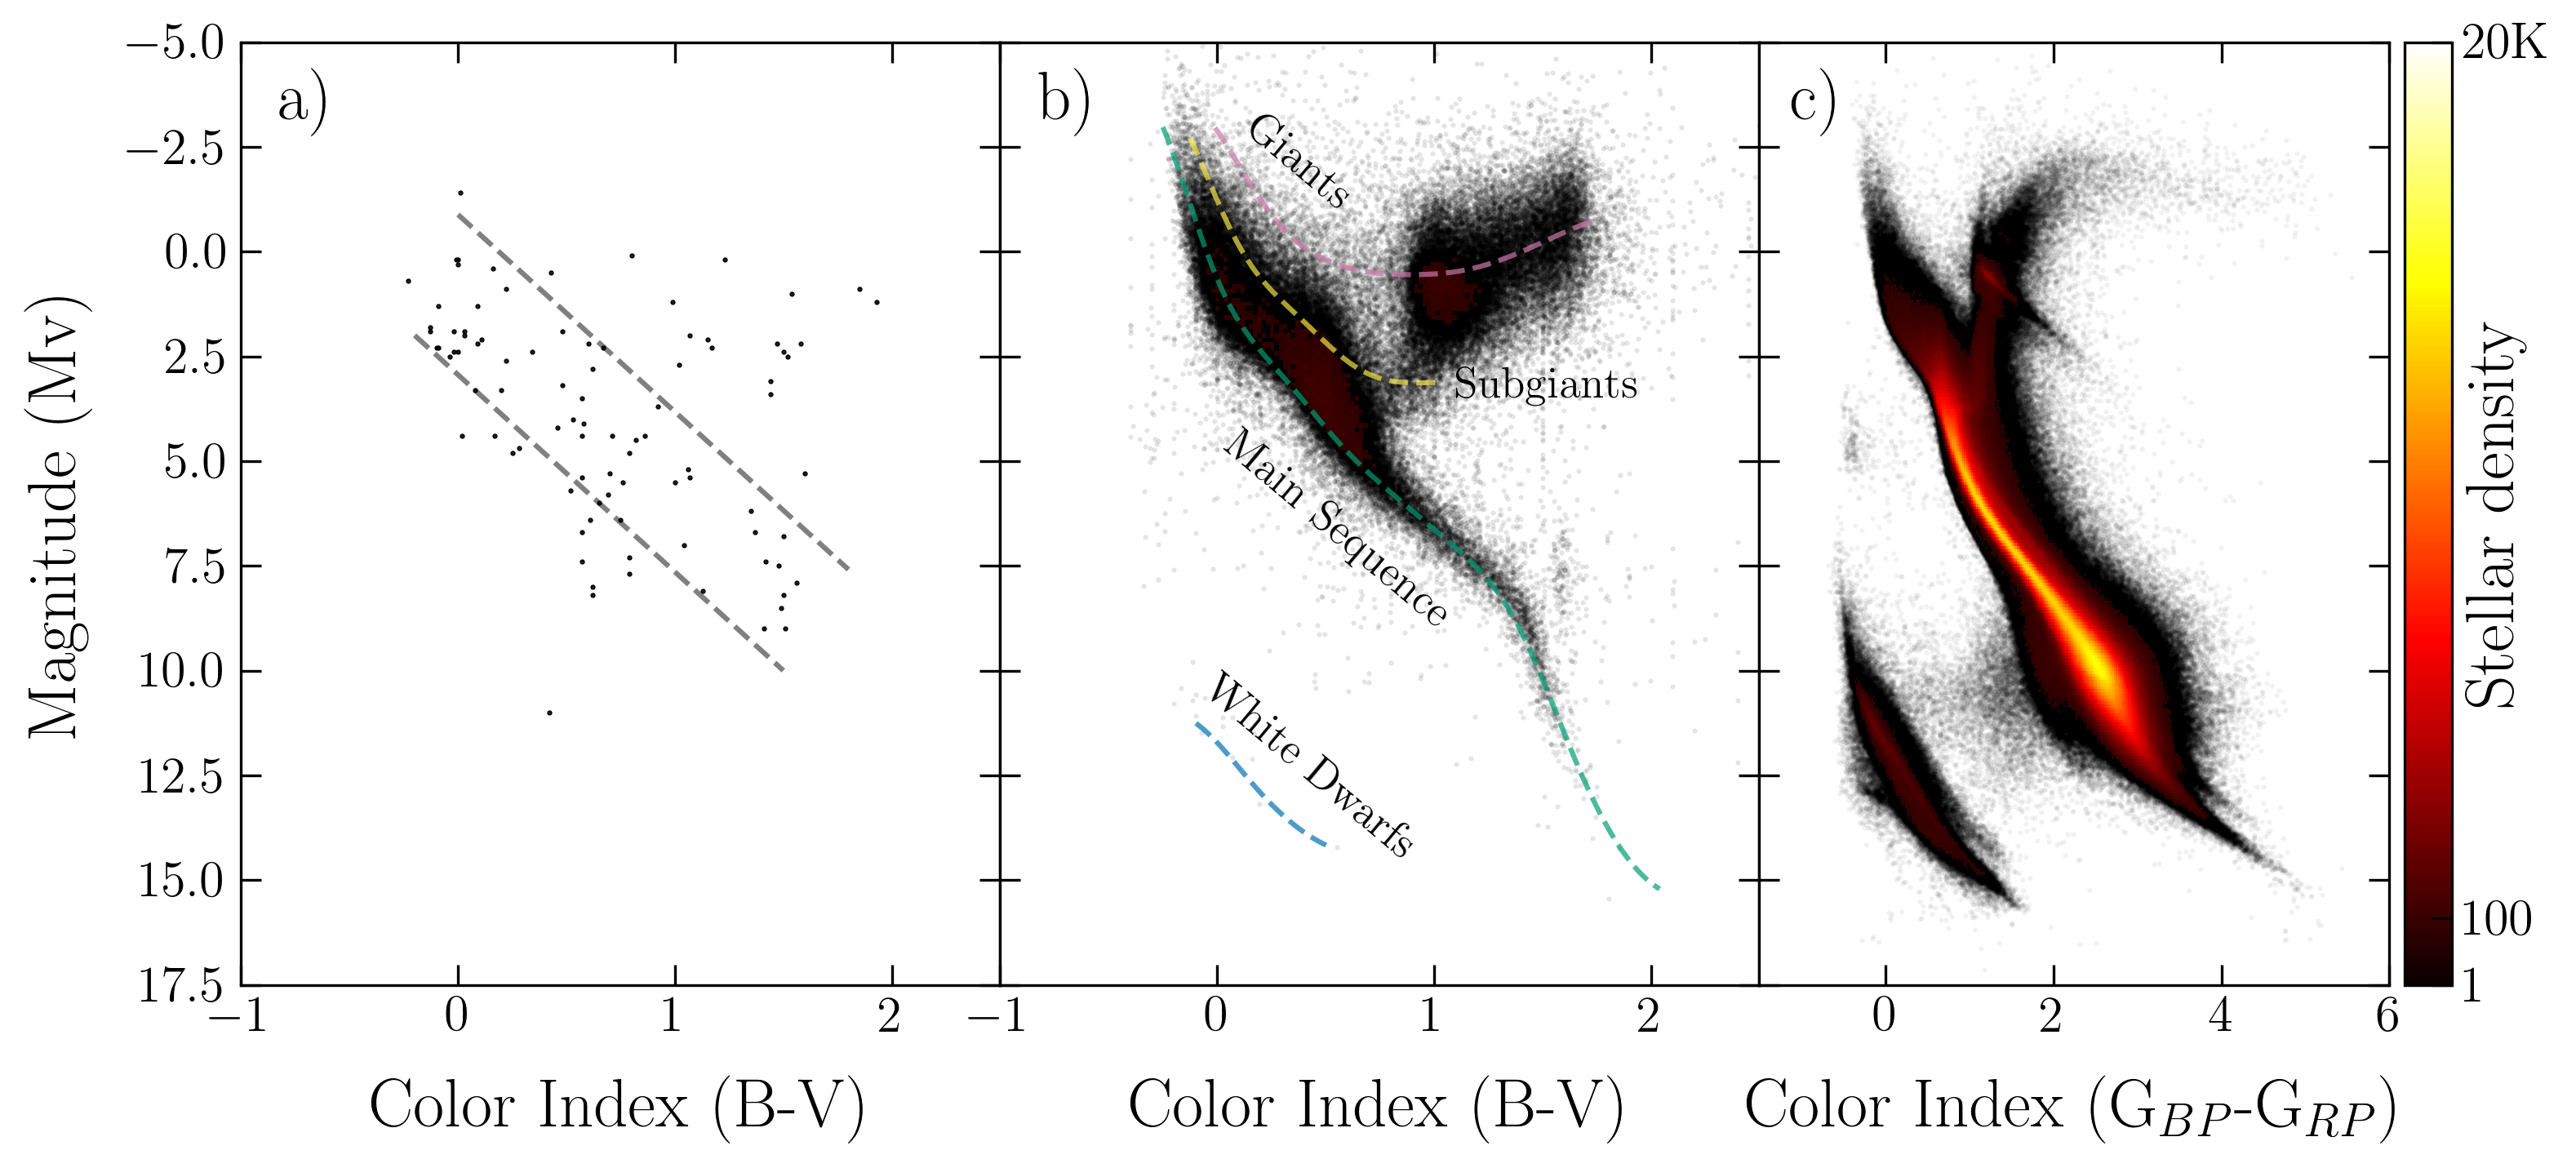
\includegraphics[width=1.2\linewidth]{figures/hr_diagram.png}}
  \caption{\textbf{HR-Diagrams through the ages:}  \github{https://github.com/avivajpeyi/hr_diagram_past_to_present}}
  \label{fig:HR-diagrams}
\end{center}
\end{figure}


With this plot Russell demonstrated that the temperature and luminosity of stars are related.
Russell noted that the great majority of the plotted stars fell in a band which ran from the upper left to the lower right.
He indicated this region with lines (the gray dashed lines reconstructed Figure~\ref{fig:HR-diagrams}(a).
Both he and Hertzsprung also noticed a separate category of bright but cool red stars in the upper right corner. 

They realised that these bright-cool red stars have a large surface area to produce high luminosity at low temperatures. 
Hertzsprung hence dubbed these as the ``giant'' stars. 
Consequently, he named the less-luminous low-temperature red stars the ``dwarf'' stars. 
Russell recognised that the red dwarfs were just the bottom end of the band of stars with within the gray lines in Figure~\ref{fig:HR-diagrams}(a). 
Hence, Russell extended the grouping of ``dwarf'' stars to the entire sequence, the sequence now known as the ``main sequence''.


For Russell the diagram provided a convenient way to illustrate his ideas about stellar evolution:
\myblockquote{The giant stars then represent successive stages in the heating up of a body, and must be
more primitive the redder they are; the dwarf stars represent successive stages in later
cooling, and the reddest of these are the farthest advanced.}{Henry Russell, 1914}

A decade later, Eddington’s mass-luminosity relation would add evidence for this evolutionary march down the main sequence.
When Eddington demonstrated that the main sequence was essentially a mass sequence it seemed to follow that the stars had to move down the main sequence as they gradually converted their active mass into
energy. 
% https://arxiv.org/pdf/1302.0862.pdf

Soon, this diagram became a cornerstone for modern astrophysics, and the concepts of stellar categories led to various advancements in our understanding of stellar physics~\citeme. 
Astronomers now know that the Hertzsprung-Russell diagram can be imagined as a stellar family portrait: stars are plotted according to their colour (on the horizontal axis) and brightness (on the vertical axis) and are grouped in different regions of the diagram depending mainly on their masses, chemical composition, ages, and stages in the stellar life cycle. 
Information about stellar distances is fundamental to calculate the true brightness, or absolute magnitude, of stars.

However, Russell's diagram from 1914 only contained a few number of stars.
Some regions of the diagram are very sparsely sampled, and the large-scale patterns one can see are limited to the main sequence and a very ill-defined giant branch. 
The fact that both Hertzsprung and Russell were able to recognize these groups is a credit to their understanding of the data.


Fortunately for us, advances in technology have created much larger samples of stars with well-measured properties. 
In 1989, the Hipparcos Satellite was launched. 
This satellite, named after Hipparchus, the ancient Greek astronomer who drew up the first accurate star map, cataloged nearly 120,000 stars in its four years of operation\footnote{Unfortunately, due to a technical malfunction an onboard motor failed to fire resulting in a highly eccentric orbit of Hipparcos around Earth, with its apogee at 36,000 kilometers from Earth and perigee a mere 500 kilometers above the Earth surface!}. 


One of the primary goals of the Hipparcos mission was to furnish high quality trigonometric parallaxes for tens of thousands of stars, in order to refine the detailed structure of the observational Hertzsprung-Russell diagram and to extend the determination of absolute magnitudes to stars significantly more luminous than about Mv="0" mag. 
These Hipparcos catalog stars with low parallax error are plotted in Figure~\ref{fig:HR-diagrams}(b). 

From the diagram, there are many more details visible than those present in the 1914 version. 

Brighter stars are shown in the top part of the diagram, while fainter stars are in the lower part. Bluer stars, which have hotter surfaces, are on the left, and redder stars, with cooler surfaces, on the right. 
The colour scale in this image does not represent the colour of stars but is a representation of how many stars are plotted in each portion of the diagram: black represents lower numbers of stars, while red, orange and yellow correspond to increasingly higher numbers of stars.

The large diagonal stripe across the centre of the graph is known as the main sequence. 
This is where fully-fledged stars that are generating energy by fusing hydrogen into helium are found. 
Massive stars, which have bluer or whiter colours, are found in the upper left end of the main sequence, while intermediate-mass stars like our Sun, characterised by yellow colours, are located mid-way. 
Redder, low-mass stars are found towards the lower right.

As stars age they swell up, becoming brighter and redder. 
tars experiencing this are shown on the diagram as the vertical arm leading off the main sequence and turning to the right. 
This is known as the red giant branch.

While the most massive stars swell into red giants and explode as powerful supernovae, stars like our Sun end their days in a less spectacular fashion, eventually turning into white dwarfs – the hot cores of dead stars. 
These are found in the lower left of the diagram.


Gaia, a follow-up mission to Hipparcos, launched in 2013 with the mission of cataloging a billion stars at an accuracy 200x better than that of Hipparcos.
This Hertzsprung-Russell diagram, obtained by a selection of stars in Gaia's second release catalogue, is the most detailed to date made by mapping stars over the entire sky, containing roughly a hundred times more stars than the one obtained using data from ESA's Hipparcos mission, the predecessor of Gaia, in the 1990s. 
This new diagram contains so much highly accurate information that astronomers have been able to identify fine details that were never before seen.

The huge leap from Hipparcos to Gaia is especially visible in the white dwarf region of the diagram. While Hipparcos had obtained reliable distance measurements to only a handful of white dwarfs, more than 35 000 such objects are included in this diagram based on Gaia data. 
This allows astronomers to see the signature of different types of white dwarfs such that a differentiation can be made between those with hydrogen-rich cores and those dominated by helium.


This increase in data is seen also in GW astro and exoplanet studies. 

\subsection{The era of Gravitational wave astronomy}

History of GW 

searches for CBC 

our IMBH study 

% Statistical inference in astrophysics is a fast-evolving field with a unique set of challenges. Broadly speaking, astrophysical observations allows us to probe fundamental physics in a way that would be impossible on Earth. The strong gravity around black holes and the extreme states of matter in neutron stars could not possibly be replicated in a laboratory and thus provide a unique way to understand the universe. However, the obvious trade- off is that these objects are far away and much of the most interesting data we record stems from faint, transient events. These transient events can in general be seen as a not controlled and not reproducible natural experiment, and thus require careful statistical treatment in their interpretation.
% At the time of writing only 50 confident gravitational-wave transients from the mergers of compact objects have been reported by the LIGO/Virgo Scientific Collaboration [20, 29], and only one optical counterpart was ever detected for GW170817, a merger of two neutron stars [277]. Still, these observations provide some of the best probes of extreme gravity in many aspects. Thus, we must analyse these events carefully and use optimal techniques to infer if their physical behaviour matches our models.

% Talk about detectors and data


\begin{figure}
\begin{center}
  \centerline{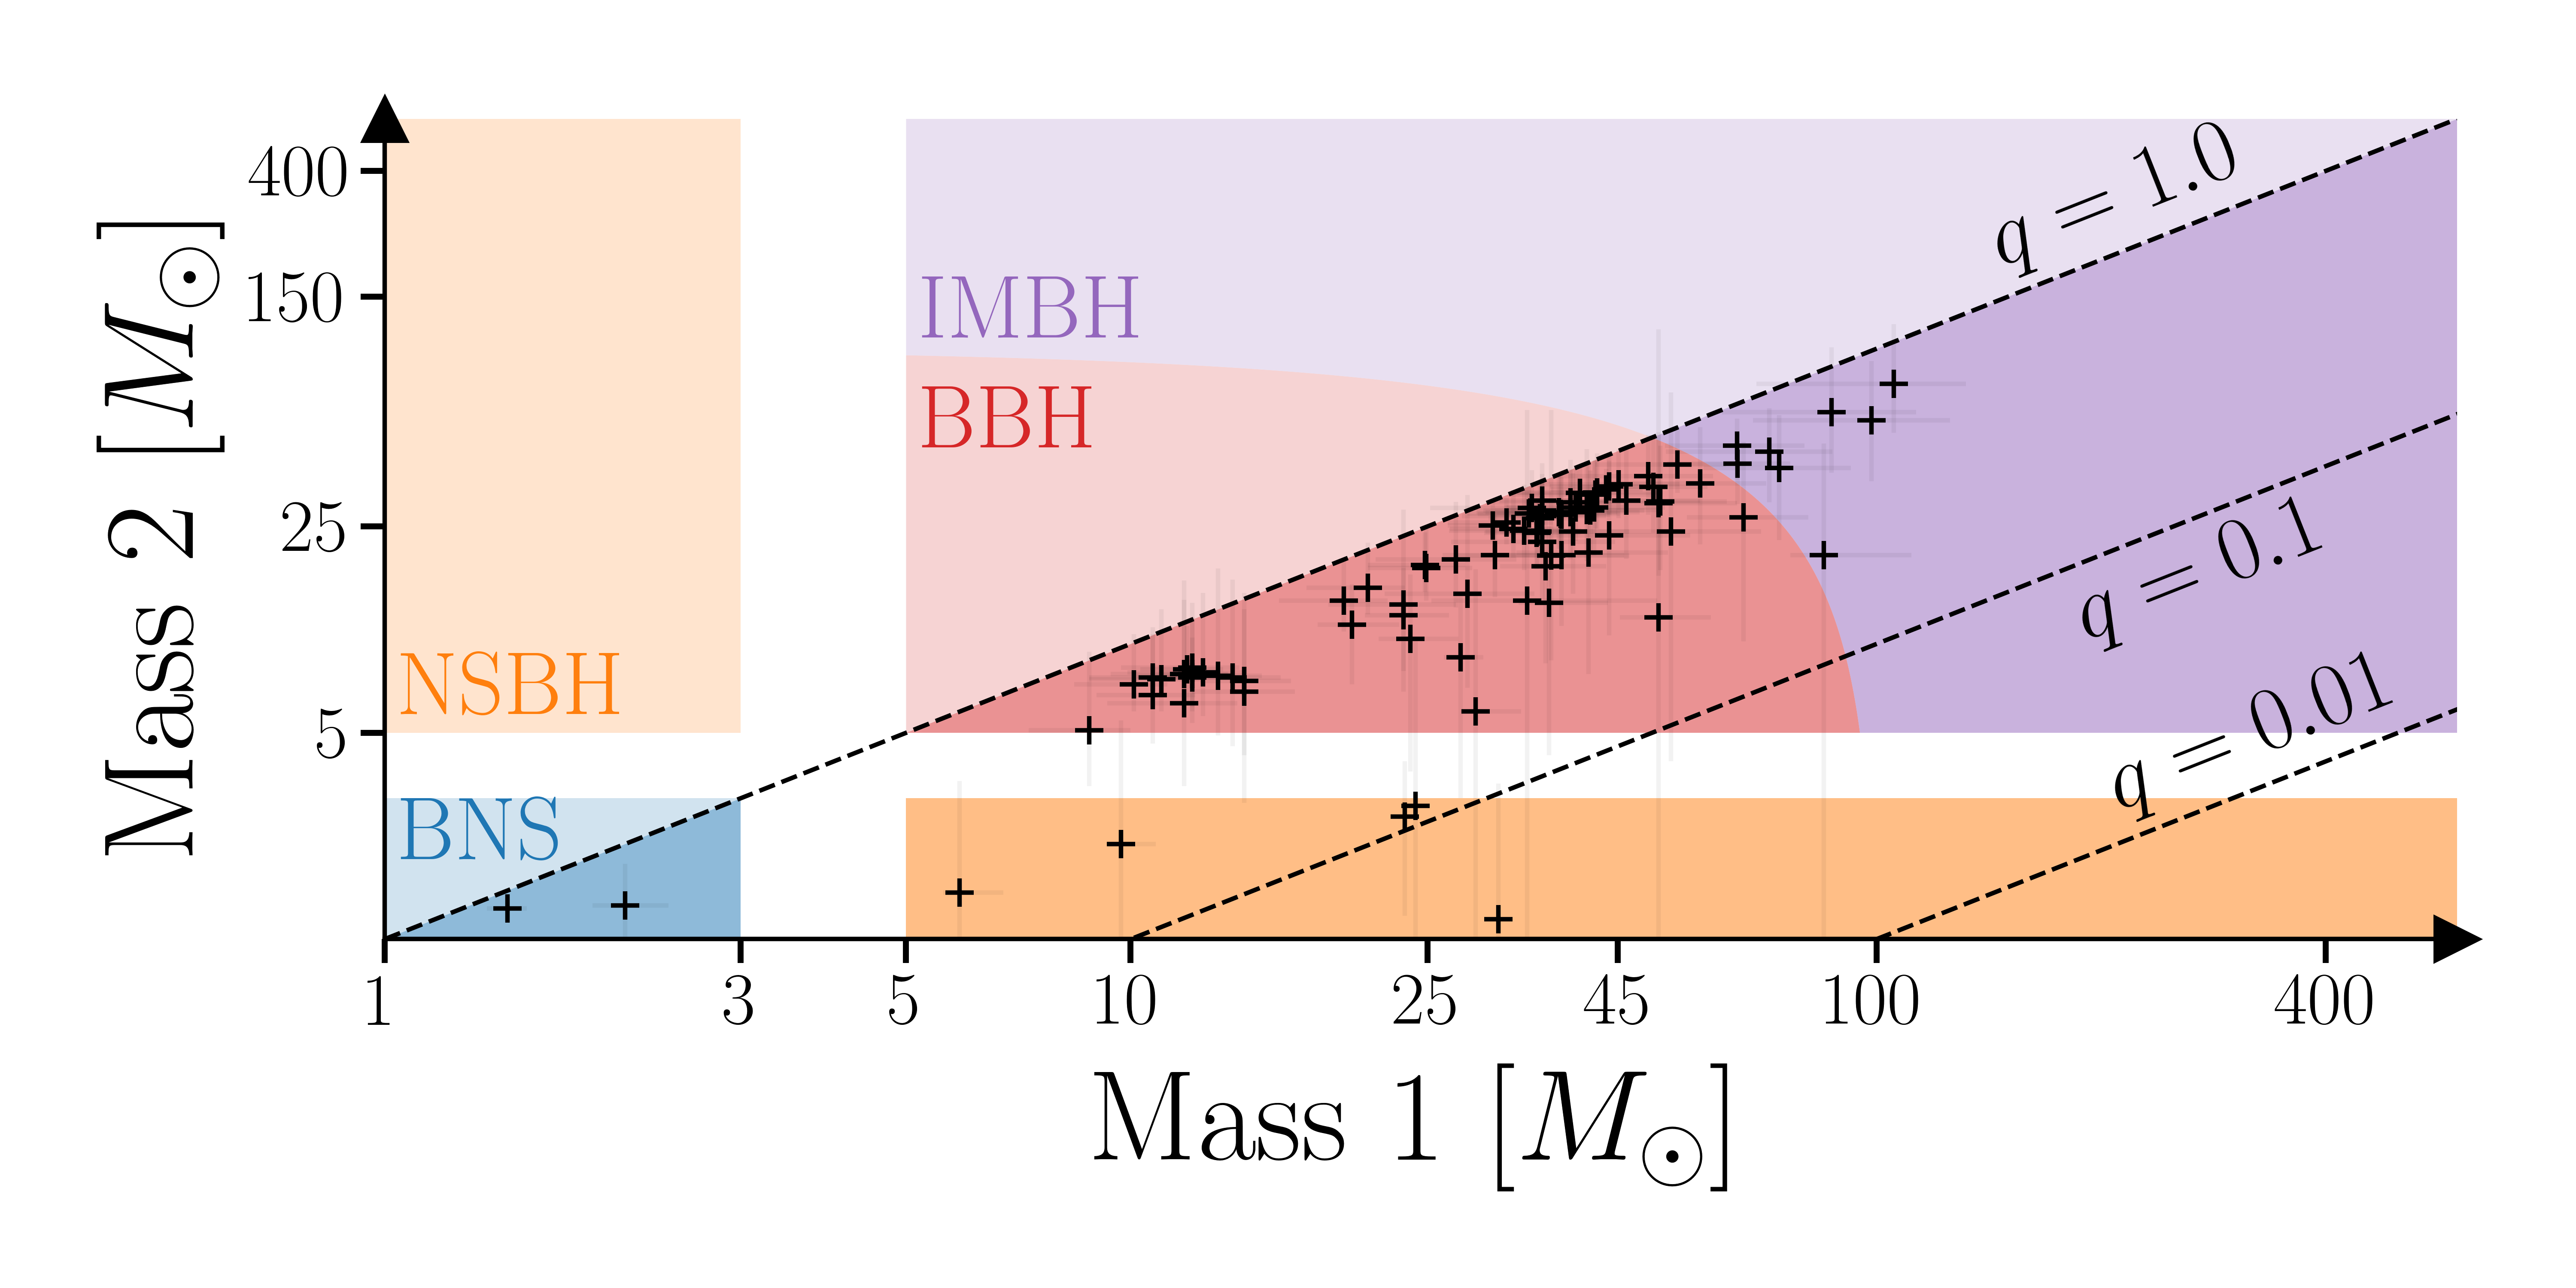
\includegraphics[width=1.1\linewidth]{src/figures/gw_catalog.png}}
  \caption{\textbf{CBC GW merger events:}  \github{https://github.com/avivajpeyi/cbc_gw_catalog_plotter}}
  \label{fig:cbc_mergers}
\end{center}
\end{figure}


\begin{figure}
\begin{center}
  \centerline{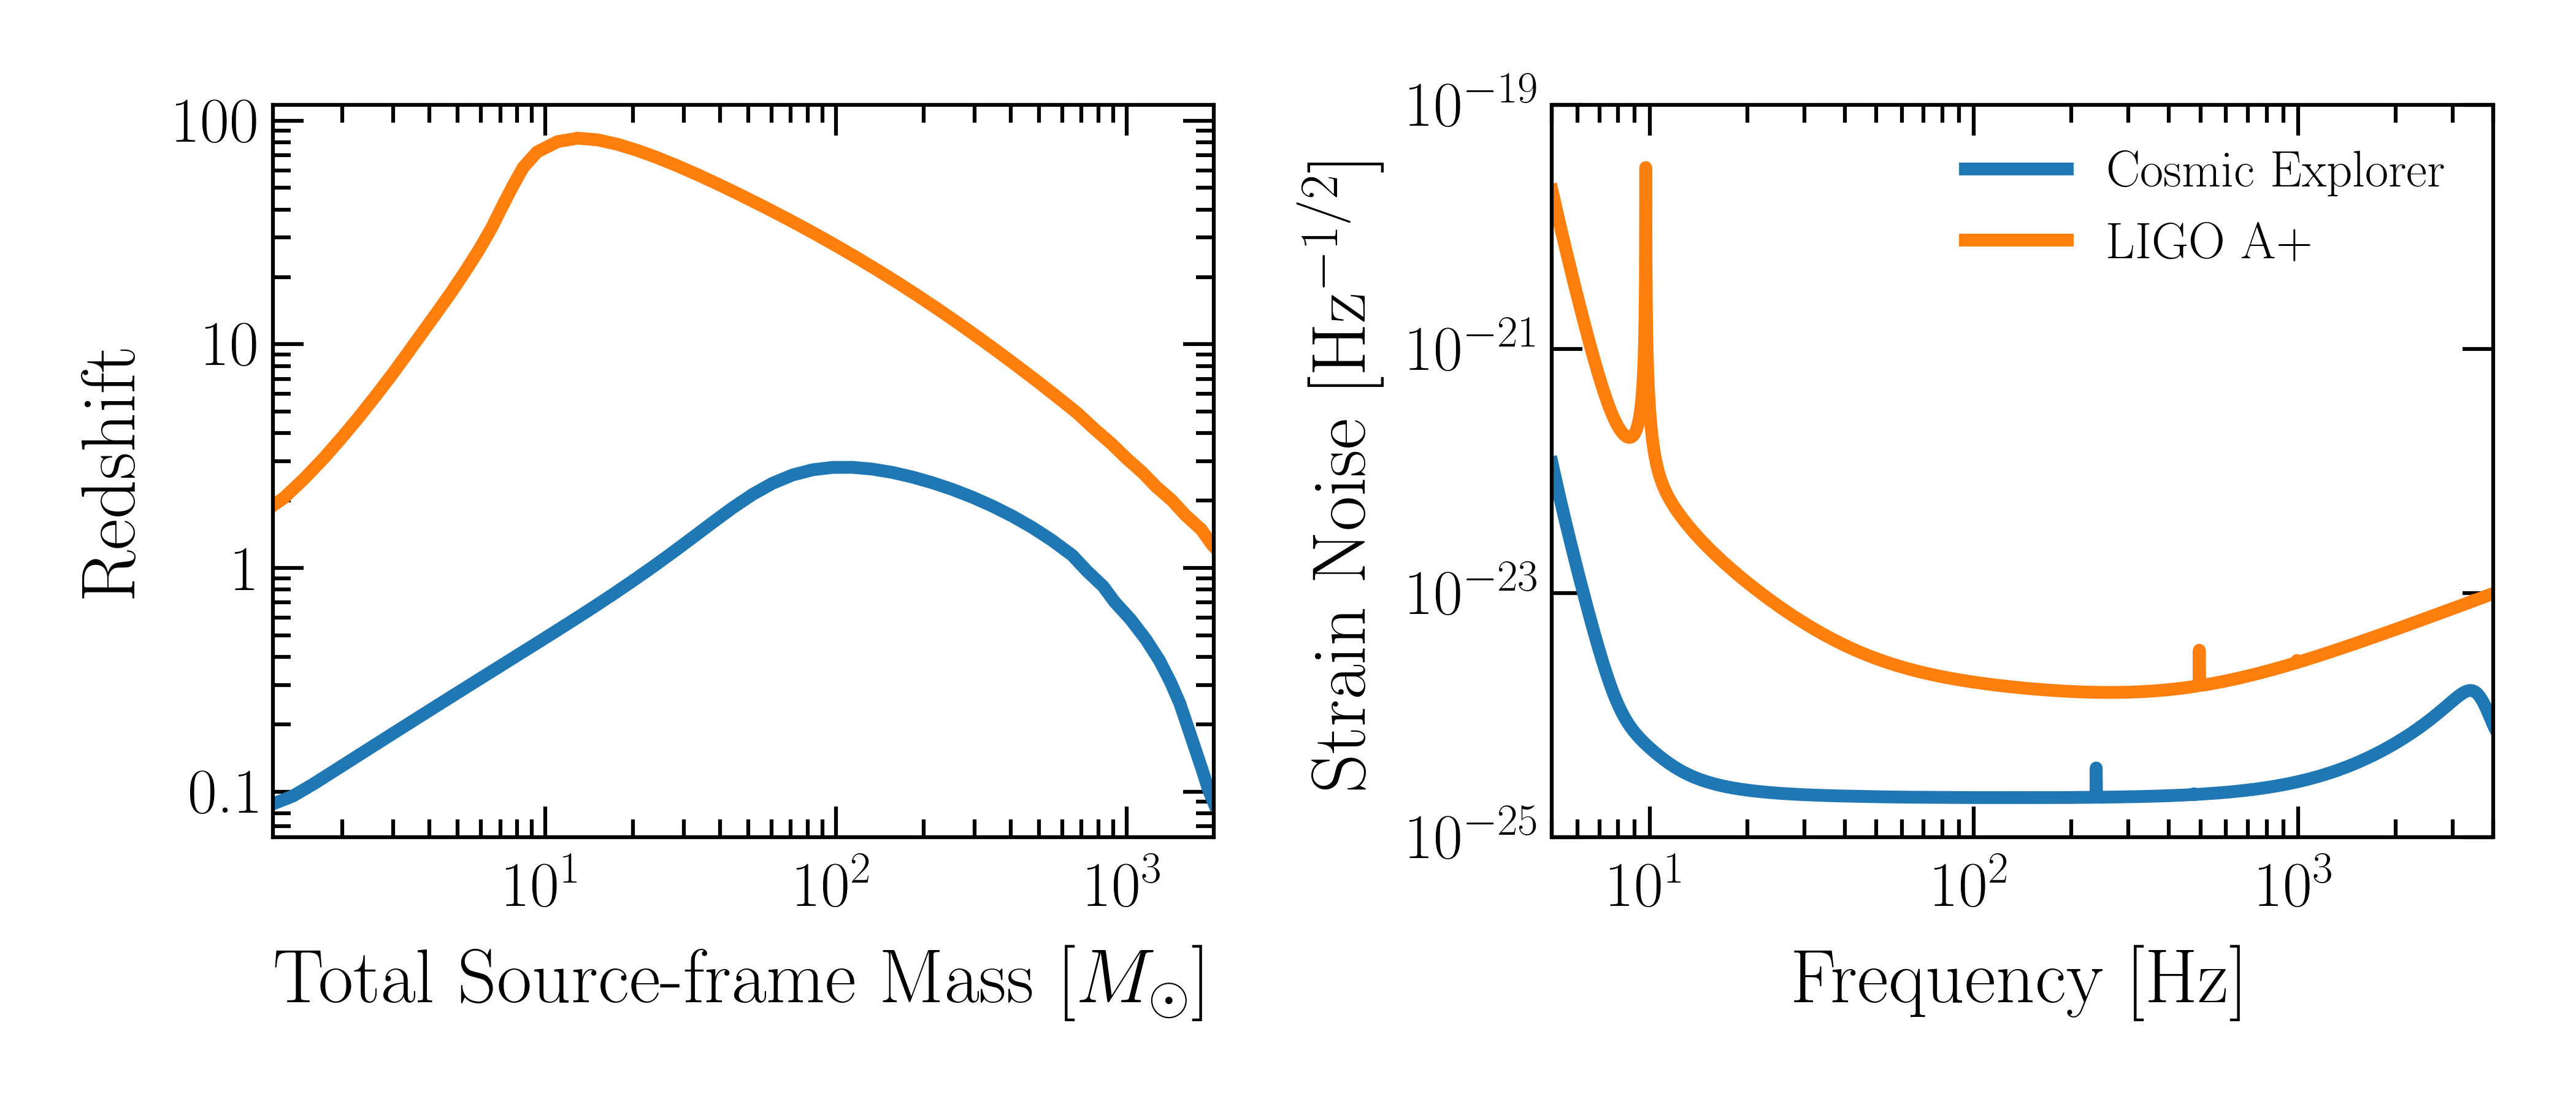
\includegraphics[width=1.\linewidth]{src/figures/ligo_vs_ce.png}}
  \caption{\textbf{LIGO A+ and CE Comparisons:}  \github{https://github.com/avivajpeyi/cbc_gw_catalog_plotter}}
  \label{fig:ligo_vs_ce}
\end{center}
\end{figure}




\subsection{The hunt for exoplanets}

We have looked for exoplanets for along time. 

First few exoplanets found 

Kepler project

now, TESS project

how the search pipelines work

Our work 


\begin{figure}
\begin{center}
  \centerline{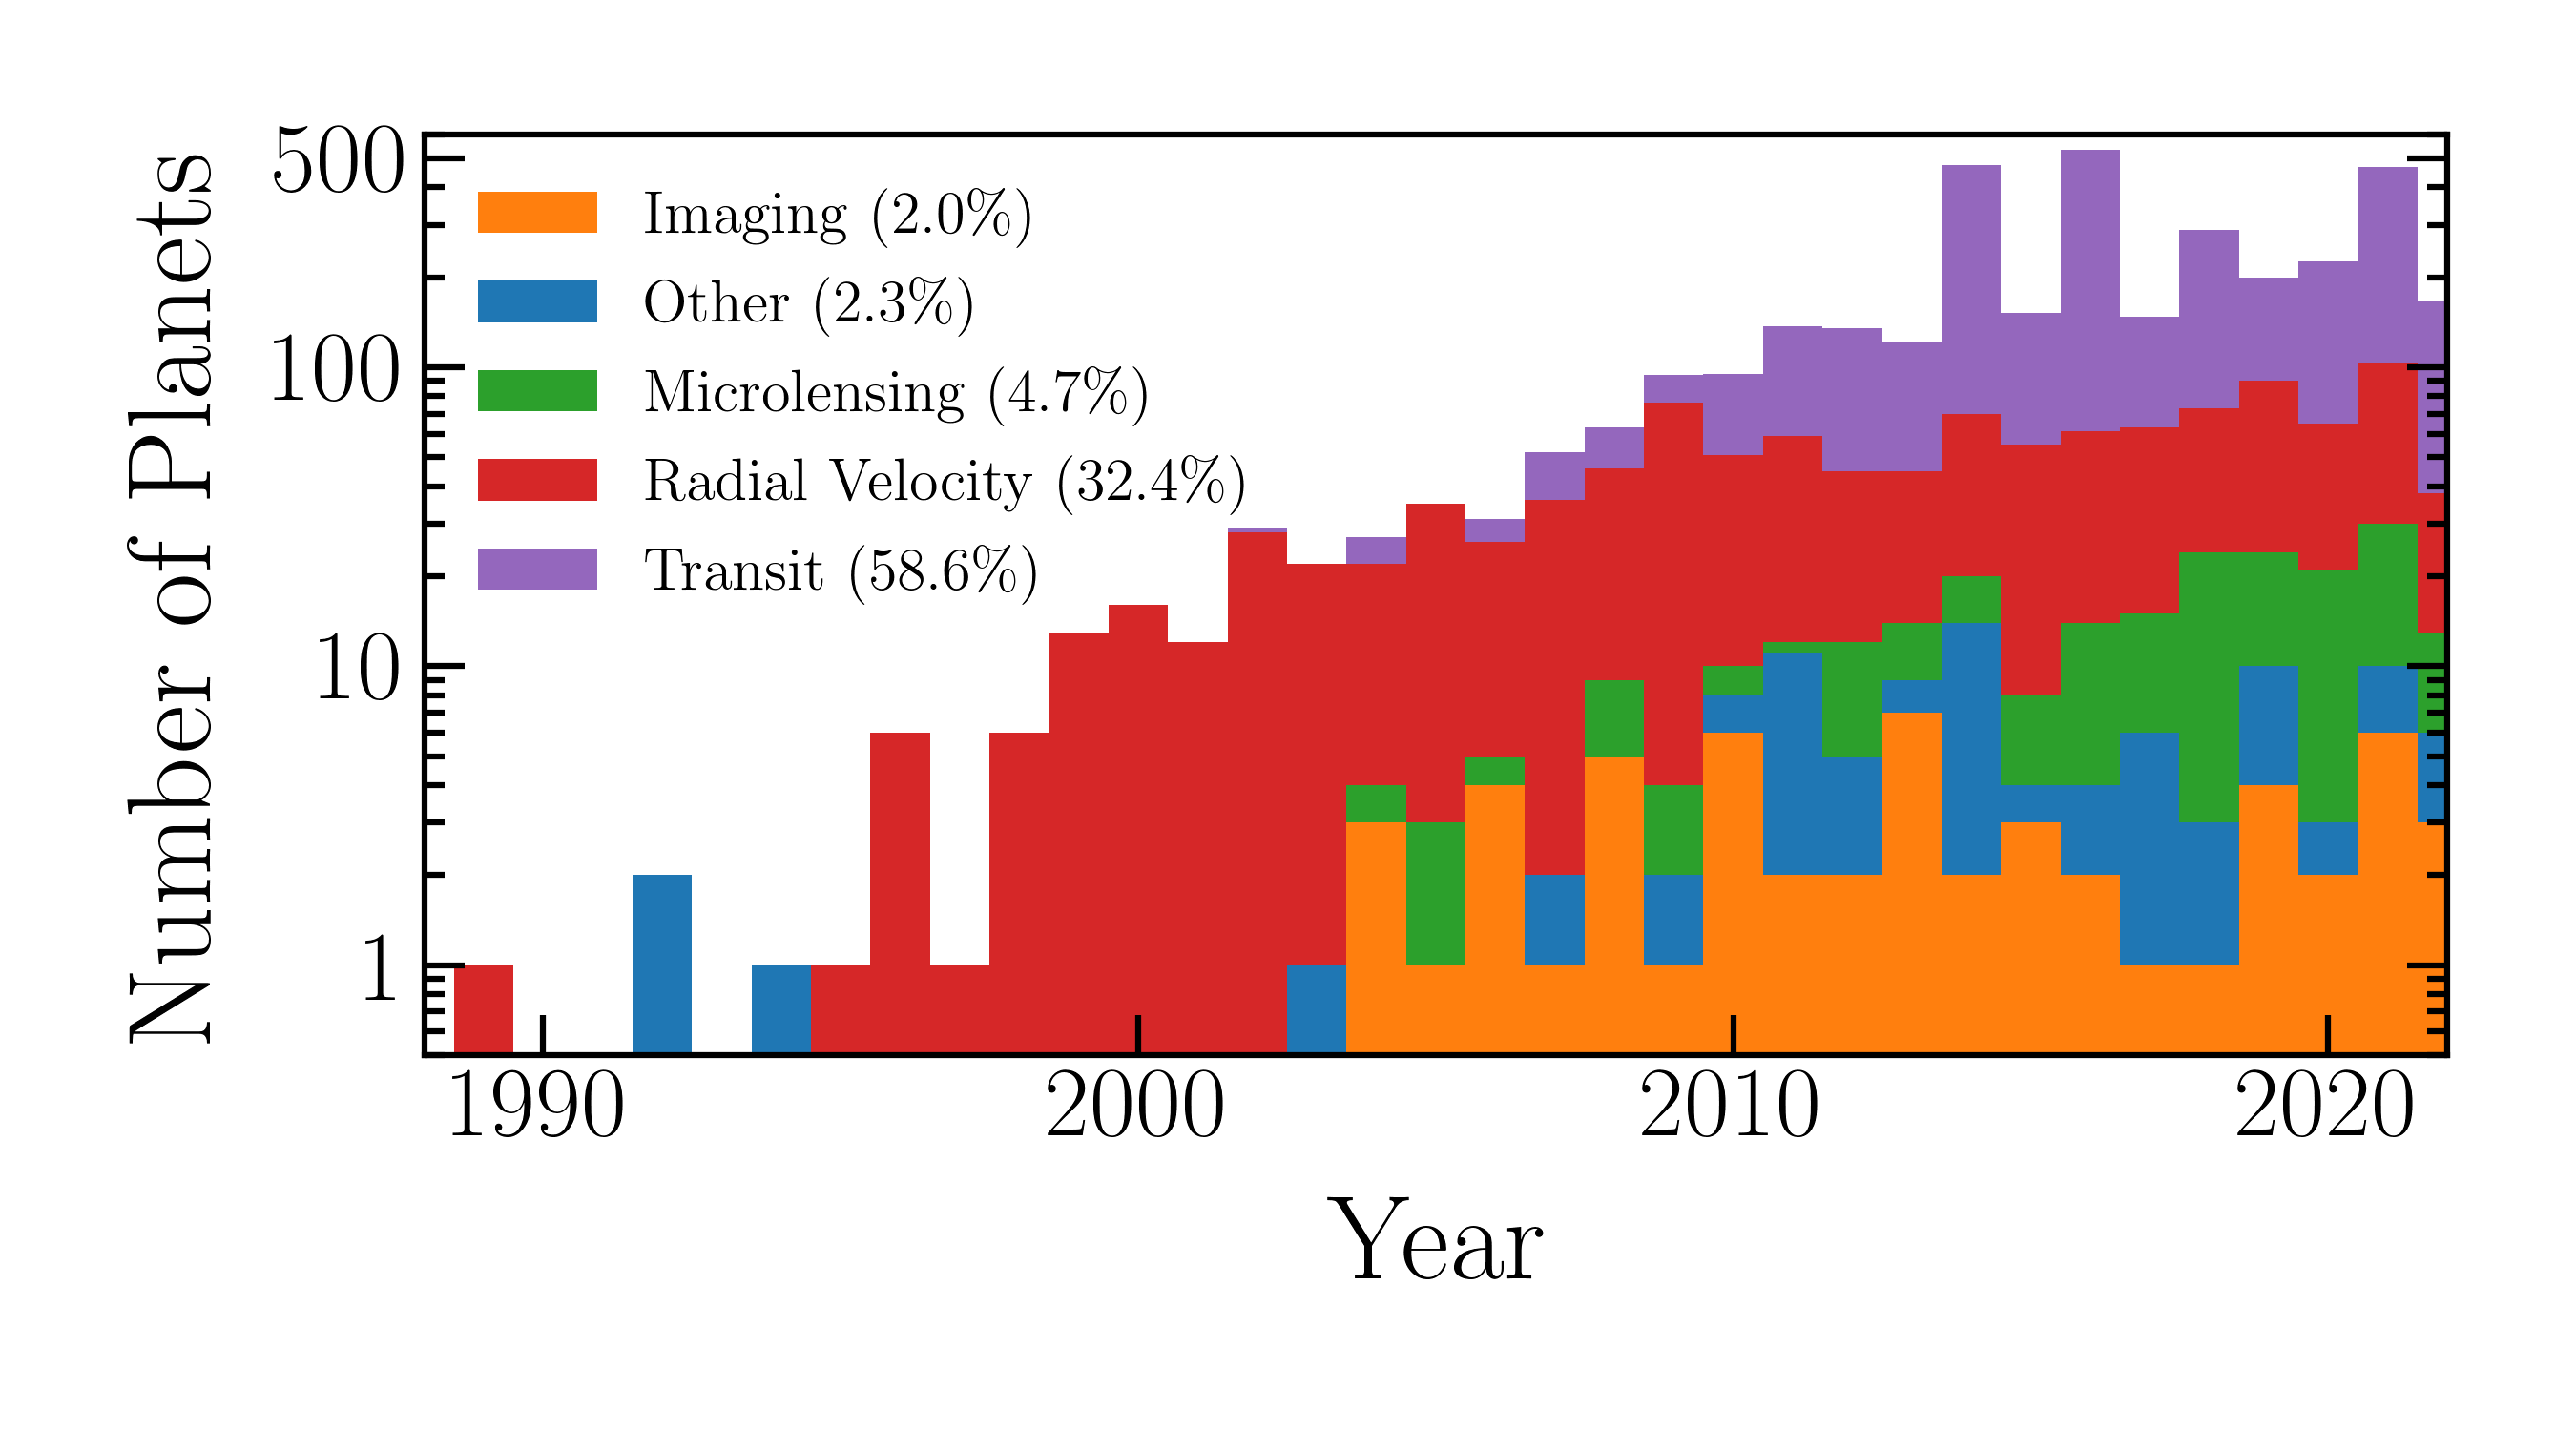
\includegraphics[width=1.\linewidth]{src/figures/confirmed_planets_vs_time.png}}
  \caption{\textbf{Exoplanet detections over time:}  \github{https://github.com/avivajpeyi/exoplanet_catalog_plotter}}
  \label{fig:exo_detections_over_time}
\end{center}
\end{figure}


\begin{figure}
\begin{center}
  \centerline{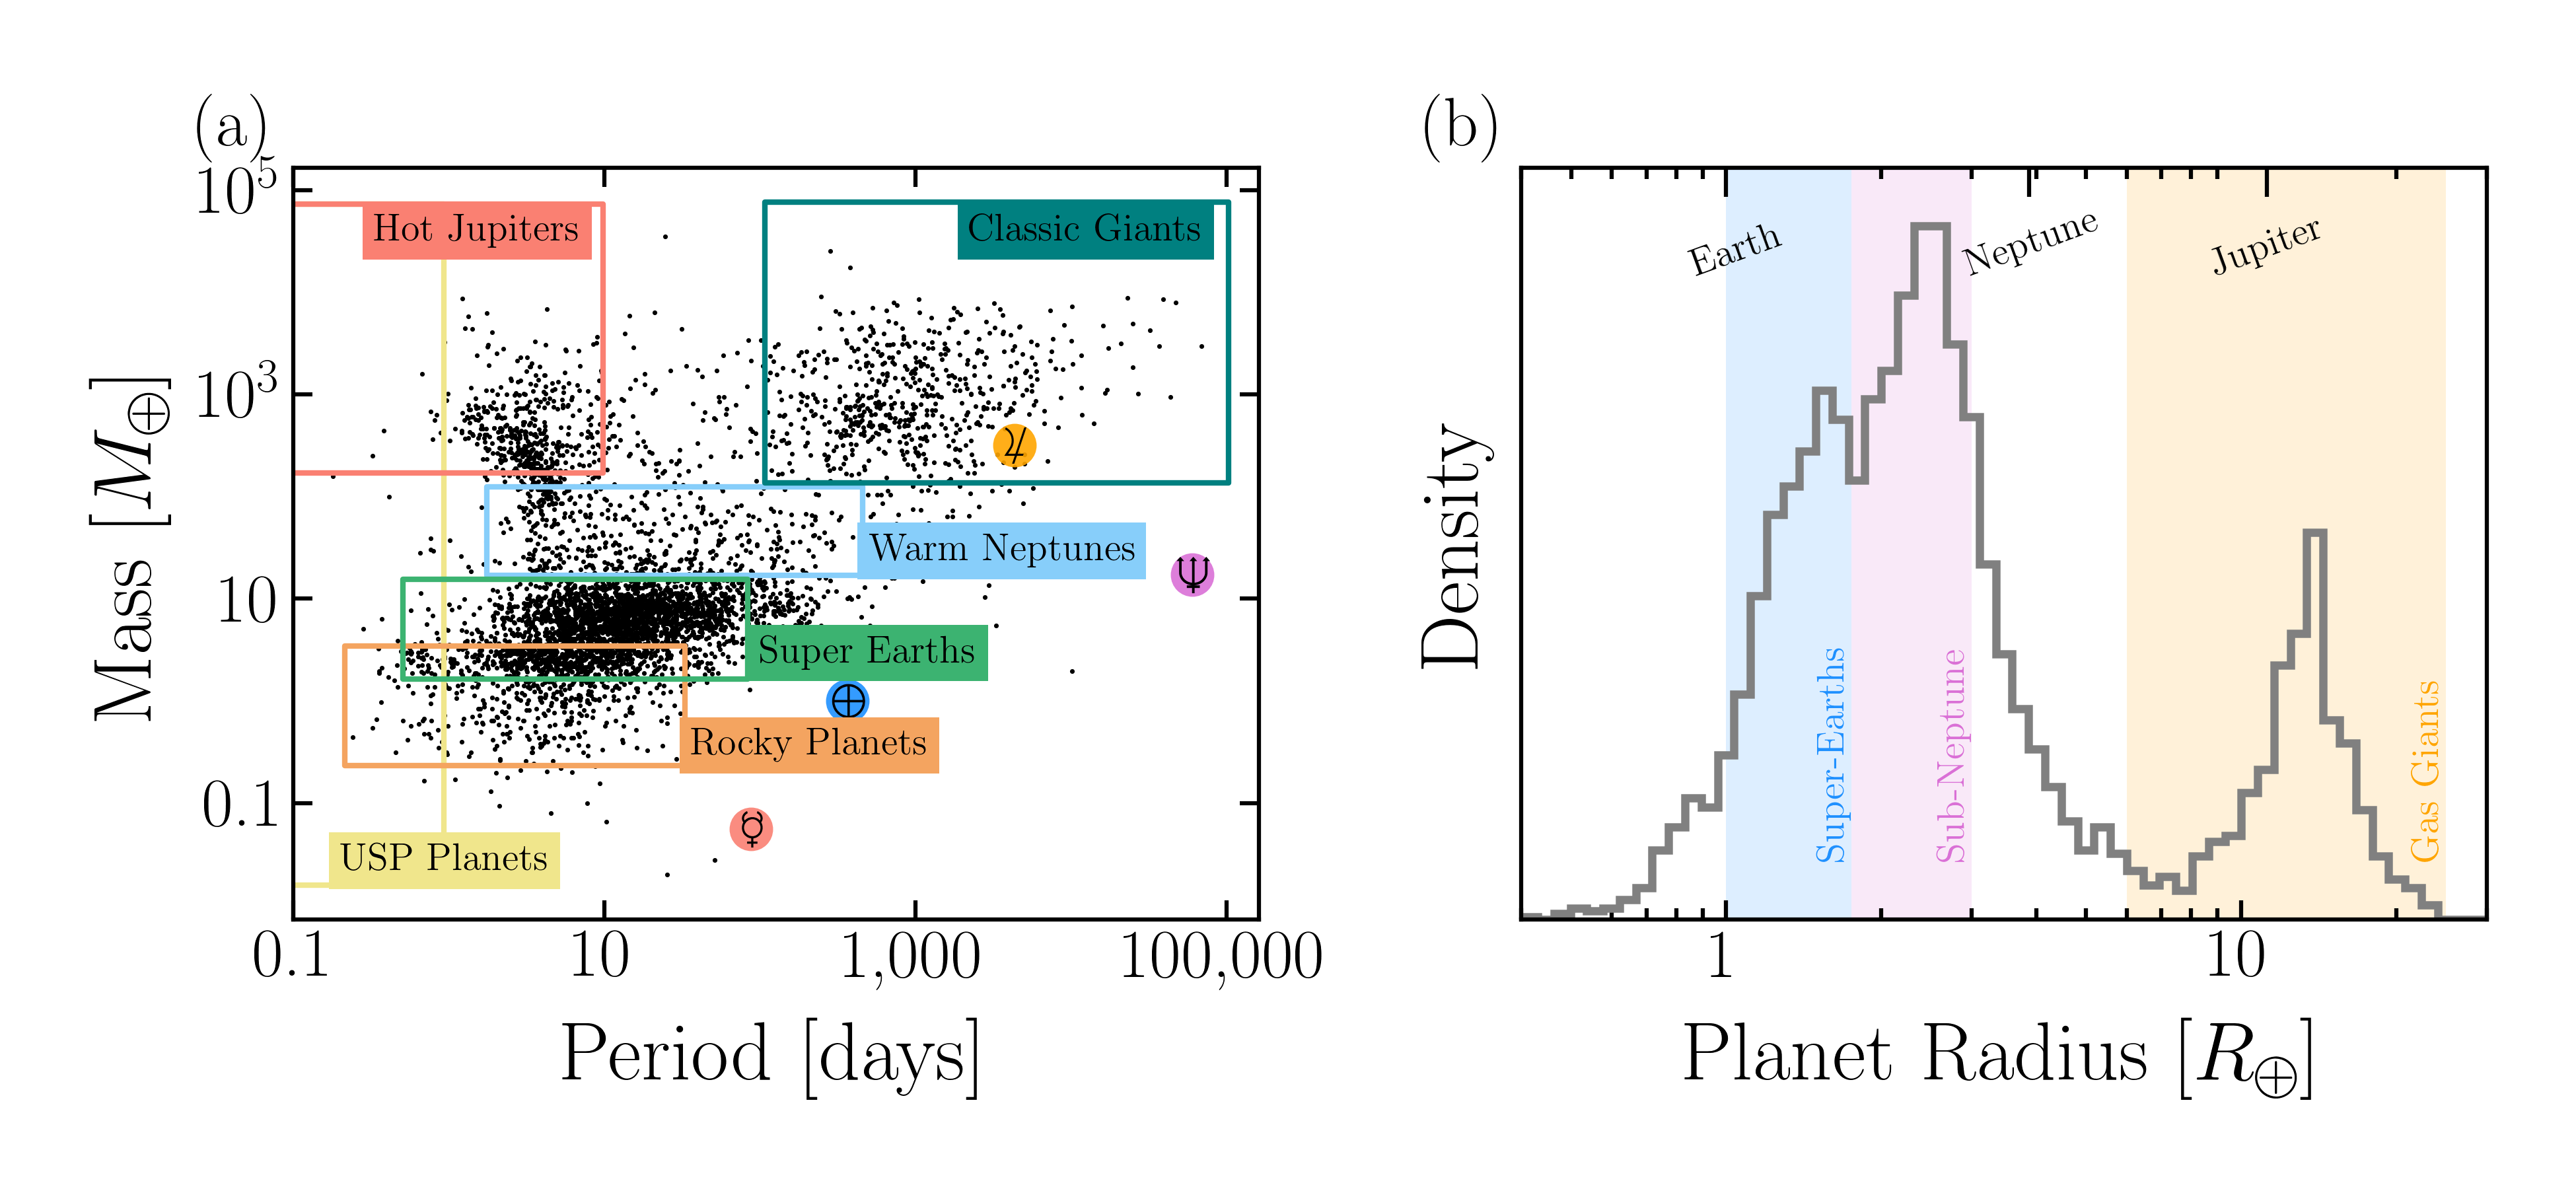
\includegraphics[width=1.\linewidth]{src/figures/scatter_categories.png}}
  \caption{\textbf{Exoplanet Categories:}  \github{https://github.com/avivajpeyi/exoplanet_catalog_plotter}}
  \label{fig:exo_categories}
\end{center}
\end{figure}


\begin{figure}
\begin{center}
  \centerline{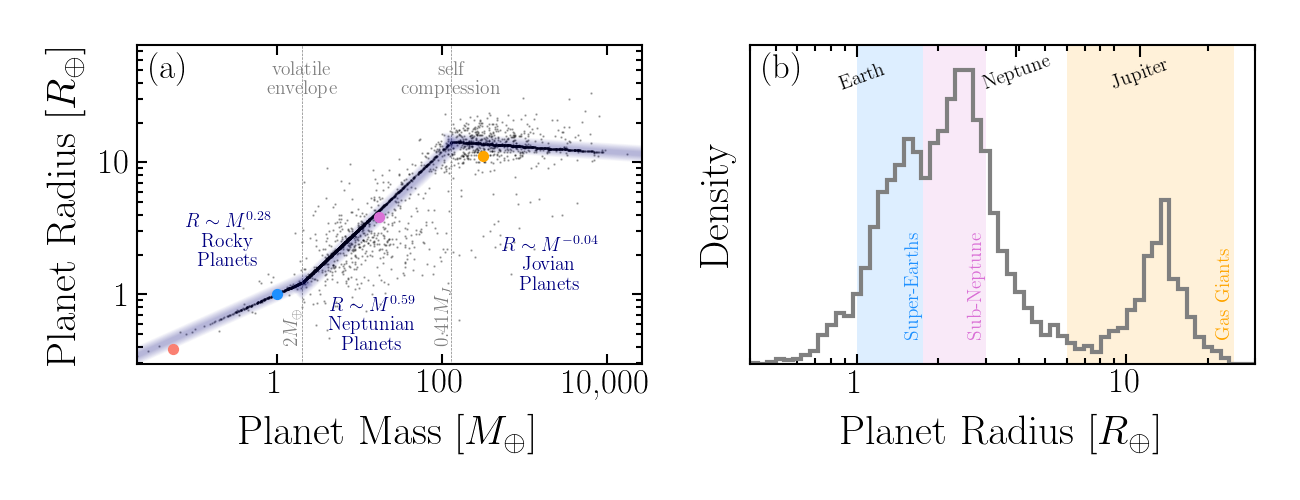
\includegraphics[width=1.\linewidth]{src/figures/radii_and_mass_relations.png}}
  \caption{\textbf{Digging into exoplanet mass and radius distributions:}  \github{https://github.com/avivajpeyi/exoplanet_catalog_plotter}}
  \label{fig:exo_mass_radius_relations}
\end{center}
\end{figure}




% Rocky vs gas 
% http://backalleyastronomy.blogspot.com/2013/07/au-dela-de-neuf-cents-exoplanetes.html


\section{Bayesian Inference}

\subsection{parameter estimation with bayesian inference}

\subsection{sampling}


\section{Gravitational Waves}




\section{Exoplanets}
